%!tex root = ../main.tex
%% Implementation
%%


%\section{Automatically proving lower bounds for LCL problems} \label{sec:implementation}
\section{Implementation} \label{sec:implementation}
In this chapter we will cover all the important topics that are used in the actual implementation.
The implementation itself is a tool, that attempts to automatically find a proof that shows the given LCL problem to be impossible to be solved in PN model (see section \ref{sec:port_number_model} for more information about PN model).
\todo{should the discussion of the implementation be after explanation of the topics?}

\subsection{The idea}
Given an LCL problem, the goal is to find a proof that it is impossible to solve the problem in PN model.
To prove this, we first assume the oppisite, that it is possible to solve the problem in PN model.
Then we try to find a counterexample that shows the assumption to be false, therefore it is impossible to solve the problem in PN model.
A graph in which we cannot find any viable labelling is a good counterexample, as this directly shows that we cannot solve the LCL problem in every graph, therefore it is impossible to solve in PN model.

For each pair of LCL problem and graph, we want to be able to check if labelling is impossible.
To perform the checking, we first encode the problem and graph into a SAT problem.
Then we leverage the power of SAT solvers to solve the SAT problem.
We feed the SAT problem into the solver, which returns either SAT (satisfiable) or UNSAT (unsatisfiable) as a result.
In case the result is UNSAT, we have found a counterexample and we are done.
Otherwise we can continue searching using some other graph.

We can repeat this routine for each graph in the current search space.
Deciding the search space is up to the end user.
A search space can be for example every graph from $n=1$ to $n=10$.
$|V| \in \{1, 2, ..., n\}$
A good strategy is to first start with small graphs and increase the size of graphs as smaller if needed.
A search space could be for example every graph 


\begin{figure}[h]
\centering
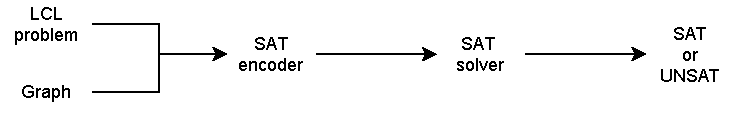
\includegraphics[]{diagrams/implementation_idea_diagram.pdf}
\caption{The process of finding negative results when given a graph and an LCL problem.}
\label{fig:implementatio:idea:1}
\end{figure}
%This is indeed what we have used in this work.
%Probably, we have to iterate a lot of graphs.
%For this purpose we want to be able to generate the graphs.




\subsection{Generating LCL-problems}
\todo{parallelization}
\subsection{Generating graphs}
\todo{parallelization}
\subsection{SAT encoding and solving}
\todo{parallelization?}
%\subsection{Software optimizations}
\subsection{Caching}
\todo{pre-computing multigraphs}
\todo{pre-computing lcl problems (and power sets of lcl problems)}
\todo{caching}

\subsection{parallelization}
\todo{Talk about parallelization here or separately in above sections}

